\documentclass[11pt]{article}

\usepackage{sectsty}
\usepackage{graphicx}
\usepackage{amsmath}
% \usepackage{gensymb}
\usepackage{graphicx}
\usepackage{accents}
\usepackage{siunitx}
\usepackage{float}
\newcommand{\sci}[1]{\times 10^{#1}}

% Margins
\topmargin=-0.45in
\evensidemargin=0in
\oddsidemargin=0in
\textwidth=6.5in
\textheight=9.0in
\headsep=0.25in

\title{ SCI238 Assignment 4}
\author{ Cosmo Zhao (20761282) }
\date{\today}
\begin{document}
\maketitle
\pagebreak
\section*{Question 1}
\subsection*{a}
% \SI[per-mode=symbol]{3.58e-12}{\watt\per\meter^2}
To determine the mass at these five points, we use the equation $M_R = v_{circ}^2 R / G$. We also conver the unit to SI by:
$$
1 kpc = 1 \sci{3} pc = 3.086 \sci{19} \SI[]{}[]{\m} \;\;\;\; 1 \SI[per-mode=symbol]{}{\km\per\s} = 1 \sci{3} \SI[per-mode=symbol]{}{\m\per\s}
$$
Then the unit is given by:
$$
\frac{(m/s)^2 \cdot m}{N\cdot m^2 / kg^2} = \frac{(m/s)^2 \cdot m}{kg \cdot m / s^2 \cdot m^2 / kg^2} = kg 
$$
For the first point:
$$
\begin{aligned}
M_R &= \frac{v_r^2 R}{G} \\
&= \frac{(20\underline{0} \sci{3})^2 \times 5.0\underline{0} \times 3.086 \sci{19}}{6.67 \sci{-11}}\\
&= 9.2\underline{5}3373313 \sci{40} kg
% &= \frac{9.2\underline{5}3373313 \sci{40}}{1.989 \sci{30}}
\end{aligned}
$$ 
For the second point:
$$
\begin{aligned}
M_R &= \frac{v_r^2 R}{G} \\
&= \frac{(25\underline{3} \sci{3})^2 \times 10.\underline{0} \times 3.086 \sci{19}}{6.67 \sci{-11}}\\
&= 2.9\underline{6}1495862\sci{41} kg
% &= \frac{9.2\underline{5}3373313 \sci{40}}{1.989 \sci{30}}
\end{aligned}
$$
For the third point:
$$
\begin{aligned}
M_R &= \frac{v_r^2 R}{G} \\
&= \frac{(26\underline{1} \sci{3})^2 \times 15.\underline{0} \times 3.086 \sci{19}}{6.67 \sci{-11}}\\
&= 4.7\underline{2}7617826 \sci{41} kg
% &= \frac{9.2\underline{5}3373313 \sci{40}}{1.989 \sci{30}}
\end{aligned}
$$
For the fourth point:
$$
\begin{aligned}
M_R &= \frac{v_r^2 R}{G} \\
&= \frac{(25\underline{9} \sci{3})^2 \times 20.\underline{0} \times 3.086 \sci{19}}{6.67 \sci{-11}}\\
&= 6.2\underline{0}7255352 \sci{41} kg
% &= \frac{9.2\underline{5}3373313 \sci{40}}{1.989 \sci{30}}
\end{aligned}
$$
For the fifth point:
$$
\begin{aligned}
M_R &= \frac{v_r^2 R}{G} \\
&= \frac{(26\underline{8} \sci{3})^2 \times 25.\underline{0} \times 3.086 \sci{19}}{6.67 \sci{-11}}\\
&= 8.3\underline{0}7678561 \sci{41} kg
% &= \frac{9.2\underline{5}3373313 \sci{40}}{1.989 \sci{30}}
\end{aligned}
$$
So at these five points, the estiamted masses are about:
$9.2\underline{5} \sci{40} kg$,
$2.9\underline{6} \sci{41} kg$,
$4.7\underline{3} \sci{41} kg$,
$6.2\underline{1} \sci{41} kg$,
$8.3\underline{1} \sci{41} kg$,
respectively.
\subsection*{b}

The loglog plot is as follows, with a linear regression line.
\begin{figure}[H]
\centerline{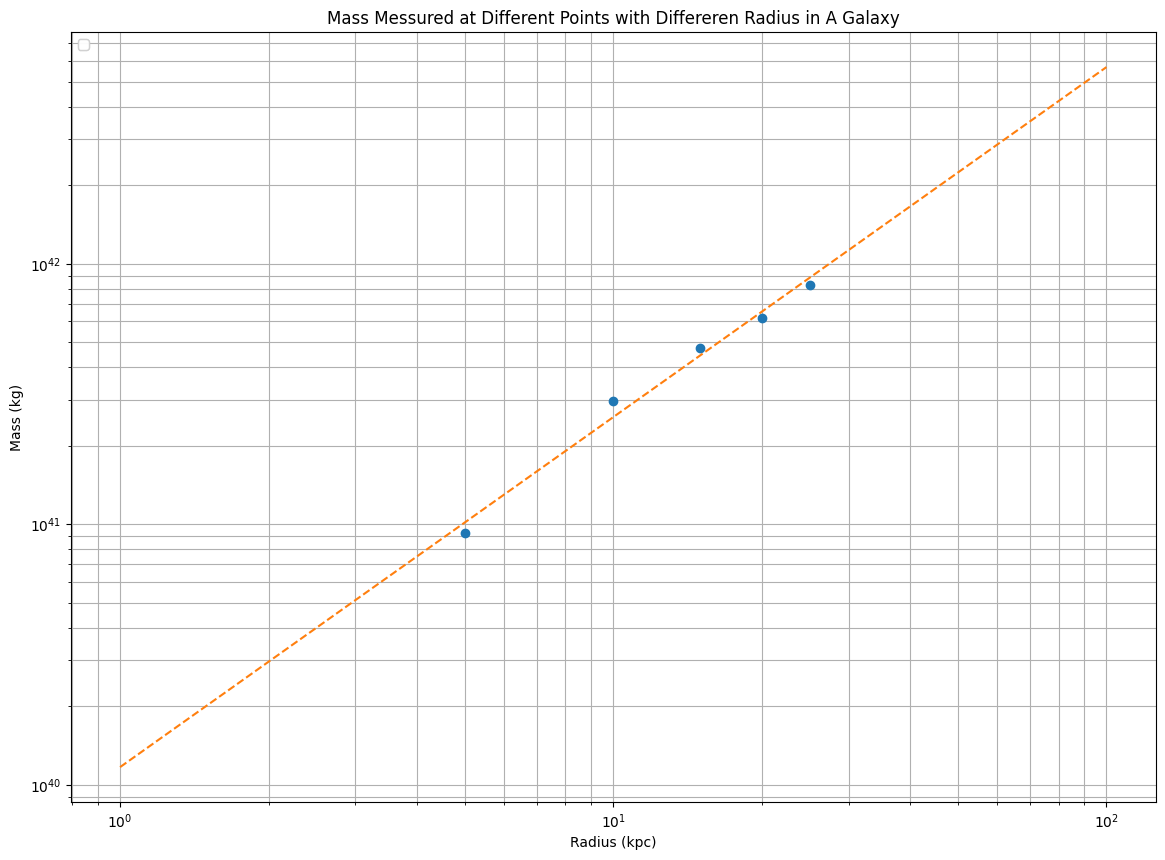
\includegraphics[scale=.5]{output.png}}
\caption{Mass measured at points in this galaxy with different radius and volocities}
\label{fig}
\end{figure}

\subsection*{c}
The picture above is drawn by matplotlib in Python.
We can see that the plotted graph roughly forms a straight line.
Then we used linear regression method with least square difference to plot the prediction line.
The parameter given by linear regression on this line is: 
slope 1.34, y-intersection: 92.3. 

Let's consider the equation given in the background:

$$
\begin{aligned}
    M_R &= 4 \pi \rho_0 R^{3-\alpha} \\
    \iff \log M_R &= (3-\alpha) \log R + \log 4\pi\rho_0
\end{aligned}
$$

In our loglog plot, y is actually $\log M_R$, x is actually $\log R$.
Therefore, with the linear regression line, we can conclude that:
$$
\begin{aligned}
    3-\alpha &= 1.3\underline{4} \\
    \iff \alpha = 1.6\underline{6}
\end{aligned}
$$
Our estimation of the value of $\alpha$ is $1.6\underline{6}$.

\section*{Question 2}

\subsection*{a}
Let's calculate the Hubble constant from each galaxy:
\begin{table}[H]
\huge
\begin{center}
\begin{tabular}{ |c|c| } 
 \hline
 A & $\frac{31\underline{0} km/s}{14.\underline{0} Mpc}
    = 22.\underline{1}4285714 \; km/(s \cdot Mpc)$\\  
 \hline
 B & $\frac{13\underline{5}0 km/s}{62.\underline{0} Mpc}
    = 21.\underline{7}7419355 \; km/(s \cdot Mpc)$\\ 
 \hline
 C & $\frac{32\underline{5}0 km/s}{14\underline{3} Mpc}
    = 22.\underline{7}2727273 \; km/(s \cdot Mpc)$\\ 
 \hline
 D & $\frac{40\underline{7}0 km/s}{18\underline{9} Mpc}
    = 21.\underline{5}3439153 \; km/(s \cdot Mpc)$\\ 
 \hline
 E & $\frac{55\underline{7}0 km/s}{26\underline{9} Mpc}
    = 20.\underline{7}063197 \; km/(s \cdot Mpc)$\\ 
 \hline
\end{tabular}
\end{center}
\end{table}
Then, let's take the average of those values to estimate:
$$
H_0 = 
 \frac{22.\underline{1}4285714 +
 21.\underline{7}7419355 +
 22.\underline{7}2727273 +
 21.\underline{5}3439153 +
 20.\underline{7}063197} {5}
 = 21.\underline{7}7700693
$$
Therefore, the Hubble Costant in this Universe should be about $21.\underline{8} \; km/(s \cdot Mpc)$.

\subsection*{b}
Since we assume constant expansion (constant velocity), the age of this universe should be the inverse of Hubble Constant
$$
\begin{aligned}
    &\frac{1}{21.\underline{7}7700693 \; km/(s \cdot Mpc)} \frac{1 \; km}{1000 \; m} \frac{3.086 \sci{22} \; m}{1 \; Mpc} \\
    = &1.4\underline{1}7090976 \sci{18} s\\
    = &1.4\underline{1}7090976 \sci{18} s \frac{1 \; yr}{31556952 \; sec} \frac{1 \; Gyr}{10^9 yr}\\
    = &44.\underline{9}0582538 \; Gyr
\end{aligned}
$$
Therefore, the age of the universe is about $44.\underline{9} \; Gyr$
\end{document}